\documentclass[thesis.tex]{subfiles}

\begin{document}

\chapter{Tumbling in turbulent flows}\seclab{tumbling}

Together with Kristian Gustavsson we investigate the orientational dynamics of small particles in random and turbulent flows. Kristian has extensive experience in studying the translational dynamics of spherical particles in random flows. In the previous Sections, describing Papers A \& B, we considered only steady and uniform fluid flows. In this project we combine our knowledge of random and turbulent flows with that of the dynamics of non-spherical particles. The collaboration has thus far resulted in Paper C (under review for publication in Physical Review Letters).

\section{Overview}

The dynamics of turbulent flow is fundamentally complicated. It is non-linear and chaotic, and reliable numerical solutions are computationally very expensive. One of the motivations for studying random flows is that, with properly chosen statistics, they may be a model system for understanding the dynamics of particles in turbulence.

This idea works well for quantities which are not crucially dependent on the specifics of turbulence. For example, one of Kristian's results concerns the relative collision velocities of particles \cite{gustavsson2013relvel}. Through a random flow model he worked out properties universal to colliding particles in any flow. In other cases, however, it turns out that the particle dynamics depends on details in the turbulent flow which are not present in the random flow. 

A random flow with a single length scale is characterised by the Kubo number $\ku = u_0 \tau/\eta$, where $u_0$ is a typical flow speed, $\tau$ a typical correlation time, and $\eta$ a typical correlation length. A small Kubo number corresponds to a rapidly fluctuating flow, with the limit $\ku\to0$ representing the white-noise limit. Large Kubo numbers correspond to steady flows.

When Parsa et. al. published numerical (DNS) and experimental results on the rotation rates of non-spherical particles in turbulence \cite{parsa2012}, they highlighted a case where the random flow predicts a qualitatively different result from the observation in turbulence. They showed that disk-shaped particles rotate, on average, about twice as fast as rod-shaped particles in turbulence. The naive prediction from a random-flow model is that disks and rods rotate alike. The questions we try to answer in Paper C are, which mechanisms are responsible for the differences in particle rotation rates? How do the statistics of the flow relate to the statistics of the particles? And what is the difference between random flows and turbulence?

It is a well-known fact that the distribution of velocity gradients in turbulent flow is strongly skewed\cite{chertkov1999,luthi2009}. We argue in Paper C that there is a relation between the skewed distribution of velocity gradients and the differing tumbling rates of disks and rods. The broken symmetry means that some flow configurations are more likely than others. We use Jeffery's equation of motion for axisymmetric particles to argue how this asymmetry propagates to the particle rotation. 

As I explained in \Secref{jefferyequation} about \emph{steady flows}, the orientational dynamics of a particle switches from rotation to alignment when one replaces a rod with a disk, or vice versa. Therefore, if rods and disks are to tumble alike on average, we must require that particles experience equal amounts of ``rotating'' gradients and ``aligning'' gradients - otherwise the result will be different if we switch the particle.
In other words, the distribution of flow gradients $\ma A$ must be symmetric over $\tr \ma A^3=0$ (see\footnote{Recall, $\ma B=\ma O + \Lambda\ma S$, but $\ma B \to \ma A$ ($-\ma A\transpose$) as the particle shape $\Lambda\to 1$ ($-1$).} \Figref{bmap} in \Secref{jefferyequation}.) This symmetry does not exist in turbulence.

However, this argument does not close the case, because it is only true for \emph{steady} flow ($\ku\to\infty$), and turbulence is absolutely not steady. The more technical part of the paper is a calculation valid at the other extreme: $\ku \ll 1$, or very unsteady flows, more so than turbulence. As shown in the paper, the calculation reinforces the picture outlined above.

It turns out that the first contribution to the rotation rate which is different for rods and disks comes from the third-order correlation functions of the flow velocity gradients. Specifically, the correlation function $\langle \ma O(0) \ma O(0) \ma S(-t)\rangle$ makes a strong contribution. Here, as throughout this thesis, $\ma O$ and $\ma S$ are the antisymmetric and symmetric parts of the Lagrangian\footnote{Along a particle trajectory; as experienced by the particle.} flow gradient matrix. The interpretation is that flow regions where there is first stretching flow ($\ma S$) and then high vorticity ($\ma O^2$) makes disks rotate, but rods align.

The manuscript is necessarily brief on some technical details, and in the following I will elaborate on two of them. First, I will show how to arrive at Eq.~(4) starting from Eq.~(3) in the manuscript. Second, I will give some detail on how we collected and verified Lagrangian statistics in a turbulent flow, along with some more data we did not find space for in the paper.

\section{Derivation of the result Eq.~(4)}

In order to derive the final result, we need to establish some facts about Lagrangian correlation functions in isotropic and incompressible flow. We denote the matrix of flow gradients by 
\begin{align*}
\ma A(\ve r(t), t) &= \nabla \ve u(\ve r(t), t),
\intertext{or in component notation}	
A_{ij}(\ve r(t), t) &= \frac{\partial}{\partial r_j}u_i(\ve r(t), t).
\end{align*}
The correlation functions between elements of a matrix $\ma A$ are denoted
\begin{align*}
	C^{AA}_{ijkl}(t_1) &\equiv \left\langle A_{ij}\left(\ve r(0),0\right)A_{kl}\left(\ve r(t_1), t_1\right)\right\rangle,\\
	C^{AAA}_{ijklmn}(t_1,t_2) &\equiv \left\langle A_{ij}\left(\ve r(0),0\right)A_{kl}\left(\ve r(t_1),t_1\right)A_{mn}\left(\ve r(t_2),t_2\right)\right\rangle,
\end{align*}
and so on. We will from now on use the shorthand $\ma A_t \equiv \ma A(\ve r(t), t)$ for brevity.
Note that we assume that the flow is statistically stationary, in the sense that the correlation between two matrix elements only depends on the time difference $t_1$, not on the particular value of $t$ (here chosen to be $0$).
We separate the gradient into its symmetric and antisymmetric parts,
\begin{align*}
	&\ma O = \frac{1}{2}(\ma A - \ma A\transpose),\quad
	\ma S = \frac{1}{2}(\ma A + \ma A\transpose),\quad
	\ma A = \ma O + \ma S.
\end{align*}
 It turns out that the all the second and third order correlation functions between $\ma S$ and $\ma O$ factorise in a very convenient manner. Appendix~\secref{applagrangian} contains the details of this factorisation and the final expressions. All the correlation functions become products of one time-dependent function, and one part which depends only on the spatial indices, but not time. For example, in three spatial dimensions
\begin{align}
	C^{OO}_{ijkl}(t) &= \frac{\left\langle \tr \ma O_0\ma O_t\right\rangle}{6}( \delta_{il}\delta_{jk}-\delta_{ik}\delta_{jl}), \nn\\
	C^{SS}_{ijkl}(t) &= \frac{\left\langle \tr \ma S_0\ma S_t\right\rangle}{30}(3\delta_{il}\delta_{jk} + 3\delta_{ik}\delta_{jl} - 2\delta_{ij}\delta_{kl}), \nn\\
	C^{SO}_{ijkl}(t) &= 0. \eqnlab{turb2point}
\end{align}
Here the functions $\left\langle \tr \ma O_0\ma O_t\right\rangle$ and $\left\langle \tr \ma S_0\ma S_t\right\rangle$ are functions of time which are flow-specific. They can be determined through a flow model, measurement, or, as in our case, numerical DNS data. See the next Section for details.

Similar, but lengthier, results exist for the eight three-point correlations $C^{SSS}_{ijklmn}(t)$, $C^{SSO}_{ijklmn}(t)$, ..., $C^{OOO}_{ijklmn}(t)$ (see Appendix~\secref{applagrangian}.)

Now we are equipped for the derivation. The dimensionless equation of motion for the particle position $\ve r$ and orientation $\ve n$ reads
\begin{align}
\dot{\ve r}&=\ku\,\ve u\,,\quad
\dot{\ve n}=\ku\left[\ma O\ve n+\Lambda\left(\ma S\ve n-(\ve n\transpose\ma S\ve n)\ve n\right)\right]\,.\eqnlab{turbeqnofmotion}
\end{align}
Here, $\Lambda$ is the particle shape function, $\Lambda=-1$ for disks, and $\Lambda=1$ for rods. The equation for $\ve r$ comes only implicitly into the equation for $\ve n$, through the dependence of $\ma O$ and $\ma S$ upon particle position.

We consider an ensemble of particles, found in the flow at a distant past time $t=0$ with initial condition $\ve n_0$. Then we compute the ensemble average of the squared rotation rate $\langle \dot n^2\rangle$ at a much later time $t$.
In the calculation we will eventually take $t\to\infty$. The average rotation rate squared is
\begin{align}
	\langle \dot n^2\rangle &= \ku^2\left\langle\left(\ma O_{t}\ve n_{t}+\Lambda\left(\ma S_{t}\ve n_{t}-(\ve n_{t}\transpose\ma S_{t}\ve n_{t})\ve n_{t}\right)\right)^2\right\rangle\nn \nn\\
	&= \ku^2\big[-\left\langle\ve n_{t}\transpose \ma O_{t} \ma O_{t} \ve n_{t}\right\rangle \nn\\
	&\qquad\qquad+ \Lambda\left\langle\ve n_{t}\transpose(\ma S_{t}\ma O_{t} - \ma O_{t}\ma S_{t})\ve n_t\right\rangle \nn\\
	&\qquad\qquad+ \Lambda^2\left\langle\ve n_{t}\transpose\ma S_{t}\ma S_{t}\ve n_{t}\right\rangle \nn\\
	&\qquad\qquad-  \Lambda^2\left\langle(\ve n_{t}\transpose\ma S_{t}\ve n_{t})^2)\right\rangle\big].\eqnlab{ndotsquared}
\end{align}
We cannot perform the average at this point, because in general the orientation $\ve n_t$ and the gradient matrices $\ma O_t$ and $\ma S_t$ have complicated joint statistics - the particles align preferentially to the gradients. 
The first approximation to the equation of motion \eqnref{turbeqnofmotion} is $\ve n(t) \approx \ve n_0 + \mathcal O(\ku)$.
%As explained above, $\ve n_0$ is uncorrelated with the flow at the later time $t$, 
The initial condition $\ve n_0$ is not a random variable, and we may average using the Lagrangian correlation functions \eqnref{turb2point}. For example,
\begin{align*}
 	\left\langle\ve n_{0}\transpose \ma O_{t} \ma O_{t} \ve n_{0}\right\rangle&=\ve n_{0}\transpose\left\langle \ma O_{t} \ma O_{t} \right\rangle\ve n_{0} \\
 	&= C^{OO}_{ijjk}(0)n_in_k\\
 	&= \frac{\left\langle \tr \ma O_t\ma O_t\right\rangle}{6}( \delta_{ik}\delta_{jj}-\delta_{ij}\delta_{jk})n_in_k\\
 	&=\frac{\left\langle \tr \ma O_t\ma O_t\right\rangle}{3} = -\frac{\left\langle \tr \ma A_t\transpose\ma A_t\right\rangle}{6},
 \end{align*}
where we also used $n_in_i=1$, and in the last step that $\langle\tr\ma A\transpose \ma A\rangle/2=\langle\tr\ma S\ma S\rangle=-\langle\tr\ma O\ma O\rangle$ in a homogenous flow (see App.~\secref{applagrangian}). In the same fashion we evaluate all averages in \Eqnref{ndotsquared} and find
\begin{align}
	\langle \dot n^2\rangle &=\ku^2 \left(-\frac{1}{3}\langle\tr\ma O_t\ma O_t\rangle +  \frac{\Lambda^2}{3}\langle\tr\ma S_t \ma S_t\rangle - \frac{2\Lambda^2}{15}\langle\tr\ma S_t\ma S_t \rangle\right) + \mathcal O(\ku^3)  \nn\\
	&= \frac{\ku^2}{3}\left(-\langle\tr\ma O_t\ma O_t\rangle +  \frac{3\Lambda^2}{5}\langle\tr\ma S_t \ma S_t\rangle\right) + \mathcal O(\ku^3)  \nn\\
	&= \ku^2\frac{\langle\tr\ma A_t\transpose \ma A_t\rangle}{30}\left(5 + 3 \Lambda^2\right)+ \mathcal O(\ku^3).  \eqnlab{ku2}
\end{align}
The limit of $\ku\to0$ is called the white noise limit. Physically it means that the flow is changing so rapidly that the instantaneous gradient is always uncorrelated with the particle orientation. There is no ``memory'', or correlation with the near past, in the system, hence the name white noise.

Now we proceed to compute the first effects of finite correlation time in the flow. In order to reach $\mathcal O(\ku^3)$, we need an expression for $\ve n(t)$.
The equation for $\ve n$ has the implicit solution
\begin{align}
\ve n_{t}&=\ve n_0\!+\!\ku\!\int_0^{t}\!\!\!\!{\rm d}t'\,[\ma O_{t'}\ve n_{t'}\!%
+\!\Lambda(\ma S_{t'}\ve n_{t'}\!-\!(\ve n_{t'}\transpose\ma S_{t'}\ve n_{t'})\ve n_{t'})]\,,\eqnlab{n_expansion}
\end{align}
The perturbation expansion is computed  to any order in $\ku$ by recursively inserting the entire right hand side of \Eqnref{n_expansion} into each occurence of $\ve n_{t'}$.
Iterating once we find
\begin{align}
\ve n_{t}&=\ve n_0\!+\!\ku\!\int_0^{t}\!\!\!\!{\rm d}t'\,[\ma O_{t'}\ve n_{0}\! +\!\Lambda(\ma S_{t'}\ve n_{0}\!-\!(\ve n_{0}\transpose\ma S_{t'}\ve n_{0})\ve n_{0})]\, + \mathcal O(\ku^2)\eqnlab{n_expansion2}
\end{align}
In principle, we could continue, however, for the present purpose, this first order expansion is enough.
We insert the expansion \eqnref{n_expansion2} into \Eqnref{ndotsquared} and find to third order in $\ku$
\begin{align*}
	\langle \dot n^2\rangle &=\ku^2\frac{\langle\tr\ma A_t\transpose \ma A_t\rangle}{30}\left(5 + 3 \Lambda^2\right) \\
	&\,\,\,+ \ku^3 \int_0^{t}\!\!\!\!{\rm d}t' \bigg[
%
	 - \left\langle\ve n_0\transpose \ma O_t \ma O_t [\ma O_{t'}\ve n_{0}\! +\!\Lambda(\ma S_{t'}\ve n_{0}\!-\!(\ve n_{0}\transpose\ma S_{t'}\ve n_{0})\ve n_{0})] \right\rangle\\
%
	 &\qquad- \left\langle [-\ve n_0\transpose \ma O_{t'}\!+\!\Lambda(\ve n_0\transpose \ma S_{t'}\!-\!(\ve n_{0}\transpose\ma S_{t'}\ve n_{0})\ve n_{0}\transpose)]
 \ma O_t \ma O_t \ve n_0 \right\rangle\\
%
&\qquad +\Lambda\left\langle\ve [-\ve n_0\transpose \ma O_{t'}\!+\!\Lambda(\ve n_0\transpose \ma S_{t'}\!-\!(\ve n_{0}\transpose\ma S_{t'}\ve n_{0})\ve n_{0}\transpose)](\ma S_{t}\ma O_{t} - \ma O_{t}\ma S_{t})\ve n_0\right\rangle\\
&\qquad +\Lambda\left\langle\ve n_{0}\transpose(\ma S_{t}\ma O_{t} - \ma O_{t}\ma S_{t})[\ma O_{t'}\ve n_{0}\! +\!\Lambda(\ma S_{t'}\ve n_{0}\!-\!(\ve n_{0}\transpose\ma S_{t'}\ve n_{0})\ve n_{0})]\right\rangle\\
%
	&\qquad+\Lambda^2\left\langle\ve n_0\transpose\ma S_t\ma S_t[\ma O_{t'}\ve n_{0}\! +\!\Lambda(\ma S_{t'}\ve n_{0}\!-\!(\ve n_{0}\transpose\ma S_{t'}\ve n_{0})\ve n_{0})] \right\rangle\\
%
	&\qquad+\Lambda^2\left\langle[-\ve n_0\transpose \ma O_{t'}\!+\!\Lambda(\ve n_0\transpose \ma S_{t'}\!-\!(\ve n_{0}\transpose\ma S_{t'}\ve n_{0})\ve n_{0}\transpose)]
\ma S_t\ma S_t\ve n_0 \right\rangle \\
&\qquad - 2\Lambda^2 \left\langle\ve n_0\transpose \ma S_t \ve n_0 \ve n_0\transpose \ma S_t [\ma O_{t'}\ve n_{0}\! +\!\Lambda(\ma S_{t'}\ve n_{0}\!-\!(\ve n_{0}\transpose\ma S_{t'}\ve n_{0})\ve n_{0})]\right\rangle \\
%
&\qquad - 2\Lambda^2 \left\langle[-\ve n_0\transpose \ma O_{t'}\!+\!\Lambda(\ve n_0\transpose \ma S_{t'}\!-\!(\ve n_{0}\transpose\ma S_{t'}\ve n_{0})\ve n_{0}\transpose)] \ma S_t \ve n_0 \ve n_0\transpose \ma S_t \ve n_0\right\rangle
%
\bigg] + \mathcal O(\ku^4)\displaybreak[3] %\\
%	
% 	&= \ku^2\frac{\langle\tr\ma A_t\transpose \ma A_t\rangle}{30}\left(5 + 3 \Lambda^2\right)\\
% 	&\,\,\,+ 2\ku^3 \int_0^{t}\!\!\!\!{\rm d}t' \bigg[
% 	-\Lambda \left\langle\ve n_0\transpose \ma O_t \ma O_t \ma S_{t'}\ve n_{0}\right\rangle\\
% 	&\quad\qquad\qquad\qquad+ \Lambda \left\langle\ve n_0\transpose \ma O_t \ma O_t \ve n_0 \ve n_{0}\transpose\ma S_{t'}\ve n_{0}\right\rangle \\
%  &\quad\qquad\qquad\qquad + \Lambda^3\left\langle\ve n_0\transpose\ma S_t\ma S_t \ma S_{t'}\ve n_{0} \right\rangle \\
% 	&\quad\qquad\qquad\qquad - \Lambda^3\left\langle\ve n_0\transpose\ma S_t\ma S_t \ve n_0 \ve n_{0}\transpose\ma S_{t'}\ve n_{0} \right\rangle \\
% 	&\quad\qquad\qquad\qquad - 2\Lambda^3\left\langle\ve n_0\transpose\ma S_t\ve n_0\ve n_0\transpose\ma S_t \ma S_{t'} \ve n_0 \right\rangle \\
% 	&\quad\qquad\qquad\qquad + 2\Lambda^3\left\langle\ve n_0\transpose\ma S_t\ve n_0\ve n_0\transpose\ma S_t\ve n_0\ve n_0\transpose \ma S_{t'} \ve n_0 \right\rangle 	
% %
% 	\bigg] + \mathcal O(\ku^4)
\end{align*}
There are quite a number of terms, but again, we can use the known three point correlation functions
%\footnote{See App.~\secref{applagrangian} for the complete expressions.} 
 to evaluate the averages. For example, 
\begin{align*}
	&\left\langle\ve n_0\transpose\ma S_t\ma S_t \ve n_0 \ve n_{0}\transpose\ma S_{t'}\ve n_{0} \right\rangle
	= C^{SSS}_{ijjklm}(0, t'-t)n_in_kn_ln_m \\
	&= \frac{\left\langle\tr \ma S_t\ma S_{t}\ma S_{t'}\right\rangle}{30} (3 \delta_{im} \delta_{kl}+3 \delta_{il} \delta_{km}-2 \delta_{ik} \delta_{lm})\\
	&= \frac{2\left\langle\tr \ma S_t\ma S_{t}\ma S_{t'}\right\rangle}{15}.
\end{align*}
Moreover, the correlation functions where two of the three matrices are evaluated at the same time have an exchange symmetry. More precisely it means, for instance, $C^{OSS}_{ijklmn}(0,\tau)=C^{SOS}_{klijmn}(0,\tau)$. This symmetry reduces the number of terms considerably, for example $\langle \ma S_t \ma O_t \ma O_{t'}\rangle = \langle \ma O_t \ma S_t \ma O_{t'}\rangle$. After averaging, the result is
\begin{align*}
\langle \dot n^2\rangle &=\ku^2\frac{\langle\tr\ma A_t\transpose \ma A_t\rangle}{30}\left(5 + 3 \Lambda^2\right) \\
	&\,\,\,+ \frac{2 \Lambda \ku^3}{5} \int_0^{t}\!\!\!\!{\rm d}t' \bigg[\frac{3 \Lambda^2}{7}\left\langle\tr \ma S_t\ma S_{t}\ma S_{t'}\right\rangle - \left\langle\tr \ma O_t\ma O_{t}\ma S_{t'}\right\rangle + 2 \Lambda \left\langle\tr \ma S_t\ma O_{t}\ma S_{t'}\right\rangle\bigg]
\end{align*}
Due to the statistical stationarity of the flow, we may translate the integrals to the form given in the manuscript, 
\begin{align*}
	\int_0^{t}\!\!\!\!{\rm d}t'\left\langle\tr \ma S_t\ma S_{t}\ma S_{t'}\right\rangle 
	&= \int_0^{t}\!\!\!\!{\rm d}t'\left\langle\tr \ma S_0\ma S_{0}\ma S_{t'-t}\right\rangle \\
	&= -\int_t^{0}\!\!\!\!{\rm d}\tau\left\langle\tr \ma S_0\ma S_{0}\ma S_{-\tau}\right\rangle \\
	&= \int_0^{t}\!\!\!\!{\rm d}\tau\left\langle\tr \ma S_0\ma S_{0}\ma S_{-\tau}\right\rangle
\end{align*}
The last step is to take the time $t\to\infty$, as advertised earlier. This concludes the derivation of Eq.~(4) in the manuscript:
\begin{align}
\langle \dot n^2\rangle &=\ku^2\frac{\langle\tr\ma A_t\transpose \ma A_t\rangle}{30}\left(5 + 3 \Lambda^2\right) \nn \\
	&\,\,\,+ \frac{2 \Lambda\ku^3}{5} \int_0^{\infty}\!\!\!\!{\rm d}\tau \bigg[\frac{3 \Lambda^2}{7}\left\langle\tr \ma S_0\ma S_{0}\ma S_{-\tau}\right\rangle - \left\langle\tr \ma O_0\ma O_{0}\ma S_{-\tau}\right\rangle + 2 \Lambda\left\langle\tr \ma S_0\ma O_{0}\ma S_{-\tau}\right\rangle\bigg]\eqnlab{eq4final}
\end{align}


\section{Turbulent flow data}

We do not ourselves have the resources to produce a numerical solution of the Navier-Stokes equations. But researchers at Johns Hopkins University (JHU) have published the data from a large direct numerical simulation\footnote{\url{http://turbulence.pha.jhu.edu/}} \cite{li2008}. The JHU database contains the velocity and pressure fields of homogenous, isotropic and incompressible turbulence. The spatial domain is a periodic box, and the data covers circa 45 Kolmogorov times, corresponding to the turn-around time of the largest eddy. 

The JHU database stores the data (\unit[27]{TB}) in a computing cluster, which we can access with a remote programming interface. We may query for the velocity and pressure fields, as well as their derivatives, at any time and position in the dataset. The JHU database provides both spatial and temporal interpolation, so to us the dataset is for practical purposes continuous.

We initialise a particle at a random position $\ve r$, with a random orientation $\ve n$, and query for the velocity field $\ve u(\ve r(t), t)$ and gradient field $\ma A(\ve r(t), t)$. Then we update the position and orientation by
\begin{align*}
	\dot {\ve r} &= \ve u(\ve r(t), t), \\
	\dot {\ve n} &= \ma O \ve n + \Lambda\left(\ma S \ve n - \ve n \ve n\transpose \ma S \ve n\right).
\end{align*}
The procedure is repeated for the entire duration of the data set. From the time series $\ma A(\ve r(t), t)$ we compute the required correlation functions, and other observables such as particle alignment with vorticity $\langle|\ve \Omega \cdot \ve n|\rangle$.


In \Figref{alignment} I show the probability distributions of particle alignment with the eigenvectors of the strain matrix $\ma S$, and the vorticity vector $\ve \Omega$. The straining direction $\ve e_1$ corresponds to the largest eigenvalue. We see that rods ($\lambda=100$ in this case) align preferentially to the vorticity, as previously observed \cite{pumir2011}. But we also see that disks ($\lambda=1/100$) have an even stronger preference to anti-align with the vorticity. The same pattern of opposite preference holds for the eigenvectors of $\ma S$. Disks prefer the compressing direction $\ve e_3$, while rods prefer the weakly stretching $\ve e_2$. None of the particle shapes correlate strongly to the strongest straining direction $\ve e_1$.

In \Figref{ndotsqr_pdf} I show the distribution of measured rotation rates for disks, rods and spheres. 
The sphere always rotates with the vorticity rate. We see that the disk experiences many more events of high rotation rates, which must be due to the effects of strain. The rod, on the other hand, not only rotates less than the disk, but it rotates much less than the sphere. It means that the rod's rotation is actually inhibited by the strain.

\begin{figure}
\makebox[\textwidth]{\centering%
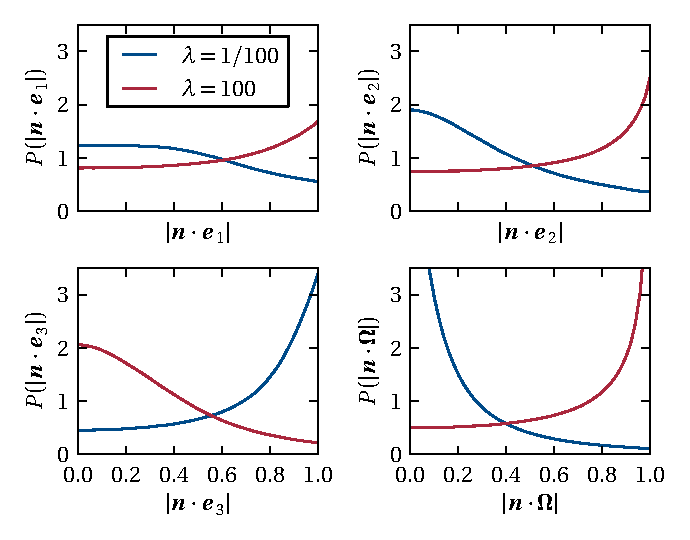
\includegraphics{figs/alignment.pdf}%
}
\caption{\figlab{alignment} Probability distributions of particle direction alignment in turbulent flow. The lower right panel shows alignment with the vorticity direction $\hat{\ve \Omega}$. The three other show alignment with the eigenvectors $\ve e_i$ of the strain matrix $\ma S$, where $\ve e_1$ corresponds to the largest eigenvalue. Red line shows distribution for a rod-shaped particle, blue line shows distribution for a disk.}%
\end{figure}

\begin{figure}
	\begin{center}
	  \makebox[\textwidth]{%
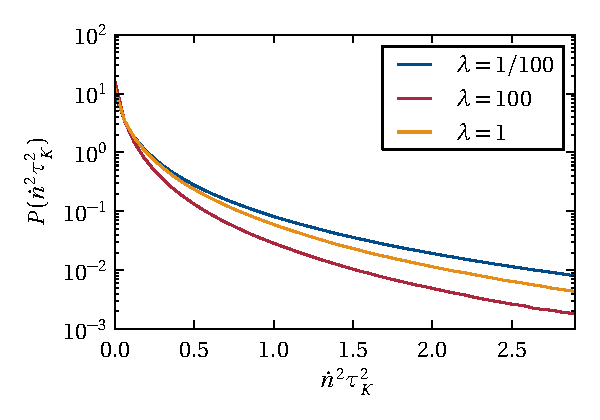
\includegraphics{figs/ndotsqr_pdf.pdf}%
}
\end{center}
\caption{\figlab{ndotsqr_pdf} Probability of observed rotation rates of a rod (red line), disk (blue line) and sphere (orange line) in turbulent flow. The peak to the far right indicates the integral over all values $\dot n^2\tau^2_{K}>3$.}%
\end{figure}

\begin{figure}
	\begin{center}
	  \makebox[\textwidth]{%
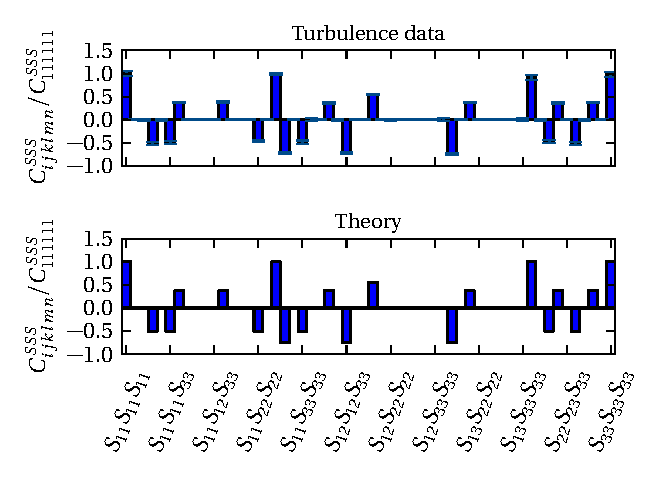
\includegraphics{figs/deltas.pdf}%
}
\end{center}
\caption{\figlab{deltas} Spatial dependence of correlation function $C^{SSS}_{ijklmn}$. Comparison between measured correlation (top) and theoretical expression \Eqnref{lagrangianSSS} (bottom). Bars are normalised by the first element. Error bars indicate one standard deviation.}%
\end{figure}

\begin{figure}
	\begin{center}
	  \makebox[\textwidth]{%
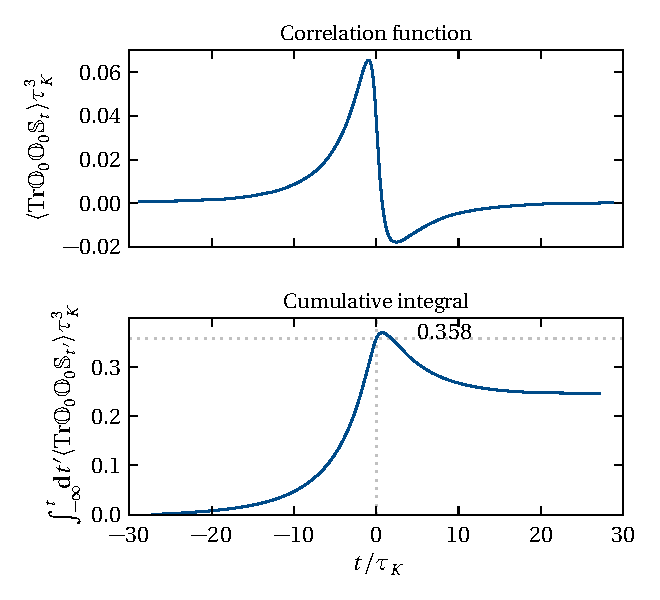
\includegraphics{figs/oosintegral.pdf}%
}
\end{center}
\caption{\figlab{oosintegral} Top panel: Time dependence of correlation function $C^{OOS}_{ijklmn}(0,t)$. Bottom panel: Cumulative integral of correlation function. The integral in the expansion for rotation rates \Eqnref{eq4final} correspond to the value at $t=0$, in this case $0.358$.}%
\end{figure}

\begin{figure}
	\begin{center}
	  \makebox[\textwidth]{%
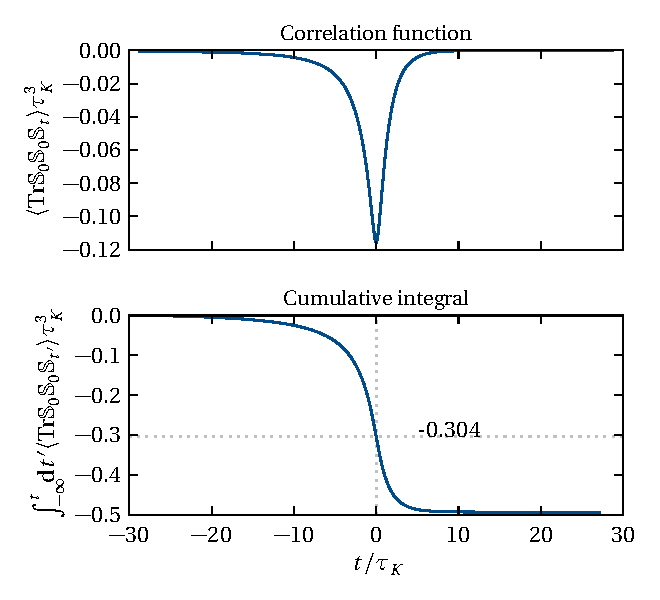
\includegraphics{figs/sssintegral.pdf}%
}
\end{center}
\caption{\figlab{sssintegral} Top panel: Time dependence of correlation function $C^{SSS}_{ijklmn}(0,t)$. Bottom panel: Cumulative integral of correlation function. The integral in the expansion for rotation rates \Eqnref{eq4final} correspond to the value at $t=0$, in this case $-0.304$.}%
\end{figure}

\begin{figure}
	\begin{center}
	  \makebox[\textwidth]{%
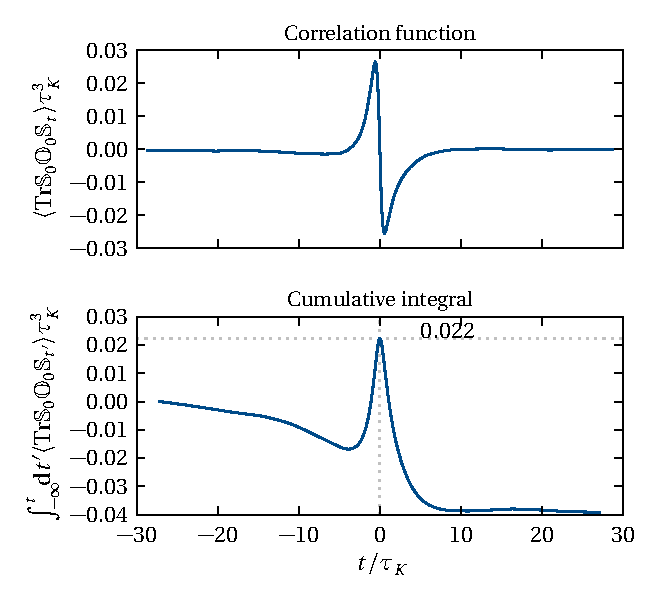
\includegraphics{figs/sosintegral.pdf}%
}
\end{center}
\caption{\figlab{sosintegral} Top panel: Time dependence of correlation function $C^{SOS}_{ijklmn}(0,t)$. Bottom panel: Cumulative integral of correlation function. The integral in the expansion for rotation rates \Eqnref{eq4final} correspond to the value at $t=0$, in this case $0.022$.}%
\end{figure}

From the data set we also compute the three integrals in \Eqnref{eq4final} in order to quantify the relative strengths of the contributions. First, we have to confirm that the correlation functions factorise according to \Eqnref{turb2point}. We compute every element of, for example, $C^{SSS}_{ijklmn}$ and compare it to the theoretical formula, in this case \Eqnref{lagrangianSSS} in Appendix~\secref{applagrangian}. The result is shown in \Figref{deltas}, and the other combinations show similar agreement with theory. We conclude that the JHU dataset indeed contains incompressible and isotropic turbulence. Second, knowing that the correlation functions factorise, we may compute the time dependence of the trace and perform the integral. In Figs.~\figref{oosintegral}-\figref{sosintegral} I show the result for the integrals relevant to the expansion \Eqnref{eq4final}.

Finally, we may use the numerical turbulence correlation functions in the expansion \eqnref{eq4final}, and compare to the numerical results of tumbling in turbulent flows. Two comments are in order. First, in turbulent flows $\ku=\mathcal O(1)$, while \Eqnref{eq4final} is valid for small $\ku$. Therefore we do not expect quantitative predictions. However, we expect the functional form of the result to be correct. That is, in this case, the dependence upon the particle shape $\lambda$. Second, in deriving \Eqnref{eq4final} we used dimensionless variables where $\ma A = u_0/\eta \ma A'$. But here we have instead expressed the correlation functions de-dimensionalised by the Kolmogorov time $\tau_{K}$, or $\ma A = 1/\tau_{K} \ma A''$. In order to proceed, we identify the time $\tau$ in the Kubo number with the Kolmogorov time $\tau_{K}$, so that $\ku \ma A'= \ma A''$. There are therefore no free parameters in \Eqnref{eq4final} when using the numerical turbulence data. The result is shown in \Figref{ndotsqr_mean}. 


\begin{figure}
	\begin{center}
	  \makebox[\textwidth]{%
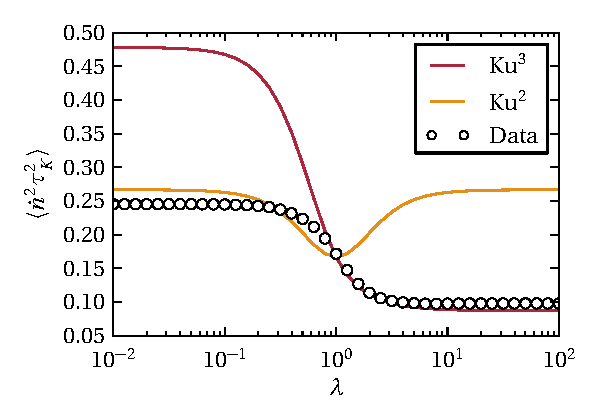
\includegraphics{figs/ndotsqr_mean.pdf}%
}
\end{center}
\caption{\figlab{ndotsqr_mean}Average rotation rate of an axisymmetric particle as function of particle aspect ratio $\lambda$. Markers show numerical results from the JHU turbulence data set. Solid lines show the small-$\ku$ expansions \Eqnref{ku2} (second order, orange line) and \Eqnref{eq4final} (third order, red line), using the correlation functions shown in Figs.~\figref{oosintegral}-\figref{sosintegral}.}%
\end{figure}









\end{document}
